\documentclass[]{standalone}

\usepackage{adjustbox}

\usepackage{amsmath}
\usepackage{xfrac}
\usepackage{mathrsfs}

\usepackage{circuitikz}
\usepackage{tikz}
\usetikzlibrary{arrows, patterns, decorations.pathmorphing, backgrounds, positioning, fit, petri, shapes, trees, matrix, chains, decorations, decorations.pathreplacing, decorations.fractals, calc,snakes,trees, decorations.markings}

\usepackage{color}
\definecolor{soton}{RGB}{7,51,71}
\colorlet{comms}{red!50!yellow}
\colorlet{payld}{pink!50!purple}
\colorlet{obdh}{green!50!black}

\begin{document}

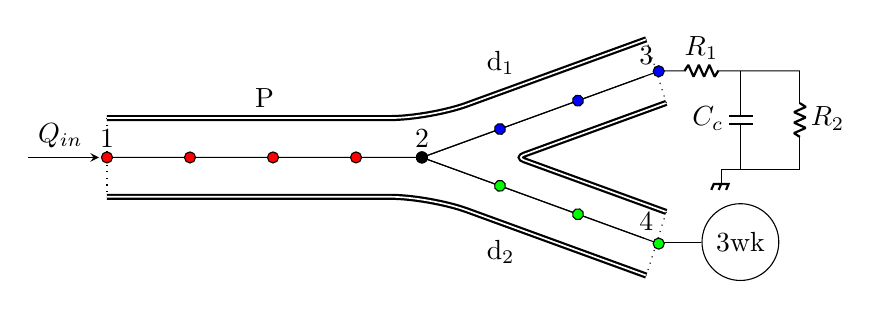
\begin{tikzpicture}[decoration={markings,
	  mark=between positions 0 and 1 step 30pt
	  with { \draw [fill] (0,0) circle [radius=2pt];}}]

		\draw[dotted] (0,0.5) -- (0,-0.5);

		\draw[double, thick, rounded corners=5mm] (0,0.5) -- (4.1,0.5) -- +(20:2.925);

		\draw (0,0) -- (4,0) -- +(20:3.2);
		\draw (4,0) -- +(-20:3.2);
		
		\node at (2,0.75) {P};
		\node at (5,1.2) {d$_1$};
		\node at (5,-1.2) {d$_2$};

		\draw[double, thick, rounded corners=5mm] (0,-0.5) -- (4.1,-0.5) -- +(-20:2.925);

		\draw[double, thick, rounded corners=1mm] ($(5.2,0)+(20:2.025)$) -- (5.2,0) -- +(-20:2.025);

		\draw[dotted] ($(5.2,0)+(20:2.025)$) -- ($(4.1,0.5)+(20:2.925)$);
		\draw[dotted] ($(5.2,0)+(-20:2.025)$) -- ($(4.1,-0.5)+(-20:2.925)$);

		\node[above] at (0,0) {1};
		\node[above] at (4,0) {2};
		\node[above] at ($(4.1,0.05)+(20:2.925)$) {3};
		\node[above] at ($(4.1,-0.05)+(-20:2.925)$) {4};
		
		
		\draw[-stealth] (-1,0) node[anchor=south west] {$Q_{in}$} -- (-.1,0);


		\ctikzset { bipoles/length=0.5cm}
		\begin{scope}[yshift=1.6cm, xshift=-1.2cm]
			\draw (8.25,-0.5) -- (8.5,-0.5) to[R=$R_1$] (9,-0.5) -- (10,-0.5);
			\draw (9.25,-1.75) to[C=$C_c$] (9.25,-.5);
			\draw (10,-0.5) to[R=$R_2$] (10,-1.75) -- (9,-1.75) node[cground] {};
		\end{scope}

		\begin{scope}[yshift=-0.575cm, xshift=-1.2cm]
			\draw (8.25,-0.5) -- (8.75,-0.5) node[circle, draw, right] {3wk};
		\end{scope}

        \path[postaction={decorate}, red, draw=black] (0,0) -- (4,0);
		\path[postaction={decorate}, blue, draw=black] (4,0) -- +(20:3);
		\path[postaction={decorate}, green, draw=black] (4,0) -- +(-20:3);
		\draw[fill=black] (4,0) circle (2pt);
		\draw[fill=black] (4,0) circle (2pt);
	    \draw[fill=blue] ($(4,0)+(20:3.2)$) circle (2pt);
	    \draw[fill=green] ($(4,0)+(-20:3.2)$) circle (2pt);
    

\end{tikzpicture}


\end{document}